\documentclass[a4paper,10pt,oneside]{article}
\usepackage[polutonikogreek,italian]{babel}
\usepackage[utf8x]{inputenc}
\usepackage{amsmath}
\usepackage{amsthm}
\usepackage{amssymb}
\usepackage{amscd}
\usepackage[pdftex,colorlinks=true,urlcolor=black]{hyperref}
\usepackage{graphicx}
\usepackage{float}
\usepackage{array}
\usepackage{rotating}
\usepackage[small]{caption}
\usepackage{lscape}
\usepackage{fancybox}
\usepackage{booktabs}
\usepackage[noanswer]{exercise}
\parindent0ex
\renewcommand{\fboxsep}{0.4cm}
\renewcommand{\textfraction}{0.05}
\renewcommand{\topfraction}{0.95}
\renewcommand{\bottomfraction}{0.95}
\renewcommand{\floatpagefraction}{0.35}
\renewcommand{\ExerciseName}{Esercizio}
\renewcommand{\ExerciseListName}{Es}
\setcounter{totalnumber}{5}
\restylefloat{figure}
\begin{document}
\section*{Elementi di geometria dello spazio}
\begin{figure}[H]
 \centering
 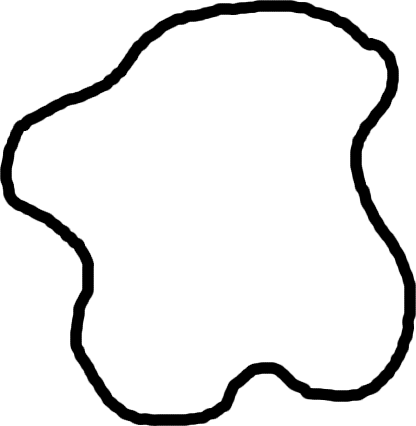
\includegraphics[width=.7\textwidth]{../immagini/superficieIrregolare.png}
 % superficieIrregolare.png
 \label{fig:superficieIrregolare}
\end{figure}



\subsection*{Lo spazio e la Fisica}
\subsubsection*{Lo Spazio, tra Fisica e Geometria}

Molti storici della Fisica sostengono che i primi studiosi ad occuparsi di Fisica in un modo paragonabile a quello dei nostri scienziati contemporanei siano stati i filosi ellenistici della Grecia antica.
Infatti, per loro, la cosidetta Geometria Euclide era, al tempo stesso, una {\bfseries teoria assiomatica} \footnote{elaborazione matematica fondata su un insieme di ipotesi astratte} e un'attività concreta di esplorazione delle proprietà dello spazio fisico. Per accettare la dimostrazione di un teorema i Greci {\slshape pretendevano} che il procedimento potesse essere visualizzato facendo uso di qualche strumento concreto, ed erano talmente fedeli a questa regola operativa che la loro è stata chiamata anche ``Geometria con riga e compasso''. 
\newline

Anche oggi, la Fisica mantiene questo atteggiamento, cercando di stabilire un confronto tra gli enti astratti della Geometria e le proprietà dello spazio reale. Per fare un esempio, se si domandasse ad un Fisico moderno di indicare un oggetto simile ad una retta, egli suggerirebbe quasi sicuramente di pensare ad un raggio di luce che viaggia nel vuoto.
\newline

Non sempre, però, il comportamento della luce si adegua alle regole della Geometria Euclidea. Esistono alcuni fenomeni nei quali la luce segue percorsi un po' sorprendenti. Consideriamo ad esempio il fenomeno dell'eclissi totale di Sole.
\newline
Durante un'eclissi totale, il disco solare non viene mai oscurato completamente, ma rimane visibile una corona luminosa molto spettacolare. Bisogna sapere, però, che il disco solare ha una dimensione più piccola di quello lunare. Ovvero, se facessimo una fotografia del sole, \footnote {usando schermi adeguati per proteggere la vista} e la confrontassimo con quella della Luna, la seconda risulterebbe più grande. Questo accade perchè i raggi solari, passando vicino alla luna, curvano assecondando la forza di gravità.
\newline

Riflettendo su questo fenomeno, Albert Einstein osservò che l'eclisse manifesta una {\bfseries {\slshape violazione}} della natura euclidea dello spazio. Infatti, un raggio di luce che, partendo dal centro del Sole fosse diretto verso il centro della Terra durante l'eclisse, potrebbe percorrere un numero infinito di strade diverse, contro il principio fondamentale per cui, {\slshape per due punti passa una e una sola retta}. 
\newline

Attualmente, la geometria euclidea è utilizzata ancora per descrivere un grande numero di fenomeni fisici e deve essere quindi ben conosciuta dagli studenti, ma è importante studiarla tenendo presente che tutte le costruzioni della matematica sono utili nel limite in cui aiutano gli uomini a descrivere in modo efficente i fenomeni osservati in concreto.

\subsection*{I vettori e le dimensioni dello spazio}
La geometria euclidea è una teoria affascinante, perché descrive lo spazio senza usare nessuna struttura di supporto.

Nelle applicazioni fisiche, però, può essere utile costruire un linguaggio più versatile, che si adatta più facilmente alle situazioni dinamiche dei fenomeni in evoluzione. Per questo motivo, molto spesso, si usano degli oggetti particolari, chiamati vettori.
\newline

Un vettore non è molto dissimile da un semplice punto dello spazio, ma aggiunge a ciascun punto dello spazio la sua relazione con un altro punto particolare, che funge da riferimento. Per questa ragione, ogni vettore possiede un {\bfseries punto di applicazione} e un {\bfseries estremo}. Un vettore si disegna come una freccia che parte nel punto di applicazione e finisce nel punto di estremo.\newline
Nel linguaggio simbolico, il vettore è indicato da un nome soprassegnato da una freccia, in questo modo: $\vec{v}$\newline
Molti testi, tuttavia, usano indicare abitualmente i vettori con un semplice simbolo in grassetto. Così: $ \mathbf{v}$ .
\newline

Ogni vettore può essere determinato indicato per mezzo di tre caratteristiche specifiche. Il {\bfseries modulo}\footnote {o intensità} , la {\bfseries direzione} e il {\bfseries verso}.\newline
Il {\slshape modulo} di un vettore è la distanza tra il vertice e il punto di applicazione.\newline
La {\slshape direzione} è la retta passante per il vertice e la coda del vettore.\newline
Il {\slshape verso} è l'orientazione del vettore, ed è diretto dalla coda verso la punta.
\newline

Due vettori che possiedono la stessa direzione, lo stesso verso e la stessa direzione sono detti equivalenti. Per riconoscere due vettori equivalenti è sufficiente riuscire a sovrapporli uno sull'altro, in modo che le rispettive punte e le rispettive code coincidano perfettamente, per mezzo di una traslazione rigida \footnote {Dunque una traslazione è rigida se conserva modulo, direzione verso del vettore}.
\newline

Come per ogni concetto della matematica, è fondamentale riconoscere le operazioni concrete che si possono definire sui vettori, per poter dire di aver capito in modo sufficiente l'argomento.\newline
Queste, per la verità, sono molto numerose, ma le principali, per i nostri scopi introduttivi, sono la {\bfseries somma}, la {\bfseries differenza} e la {\bfseries scomposizione}.\newline

Per sommare due vettori tra loro, è sufficiente trasportare, con una traslazione rigida, la coda del primo dei due sul vertice del secondo. Il vettore somma è uguale a quel vettore applicato nel punto di applicazione del secondo vettore e terminato nel punto di estremo del primo vettore \footnote {vedi disegno da integrare}. Come la geometria euclidea spiega bene, l'effetto di una somma di vettori rappresenta la diagonale del quadrilatero costruito sui i due vettori addendo.\newline
\newline

La {\slshape differenza} è l'operazione inversa della somma. In matematica, per affermare che 7 meno 3 fa 4, si deve prima verificare che 4 + 3 faccia 7. Ma
un secondo modo molto efficente per calcolare una differenza è di applicare la tecnica del resto dal rigattiere.\newline
Se, dovendo acquistare un prodotto che vale, ad esempio, venti euro, un cliente porge una banconota da cinquanta, il negoziante calcola il resto contando a partire da venti, fino ad arrivare a cinquanta.
Allo stesso modo, per fare una differenza tra un vettore  dato e un secondo, è sufficiente tracciare un vettore con il punto di applicazione coincidente con l'estremo del secondo vettore (quello sottratto) e il punto d'arrivo coincidente con il vettore dato.\newline
Come verifica, si può sommare il vettore sottratto alla differenza appena calcolata e constatare che si riottiene sempre il vettore iniziale.\newline
La differenza tra vettori è uno strumento molto efficace per rappresentare lo {\slshape spostamento} tra due punti.\newline
Osservando il parellogramma costruito su una coppia di vettori, si può osservare che la loro differenza corriponde alla sua diagonale trasversa, e biseca vicendevolmente il vettore somma.
\newline

La scomposizione, invece, è l'operazione che permette ai vettori di rappresentare le dimensioni dello spazio.\newline
Lo spazio della geometria, infatti, è un ente tridimensionale, che si estende in lunghezza, larghezza e profondità.\newline
Tuttavia, per gli scopi di questo manuale, tutte le applicazioni saranno ridotte alle due dimensioni dello spazio piano, salvo diversa indicazione.
\newline

Date due rette incidenti, che vengono dette anche {\bfseries \slshape {direttrici}} del sistema, e un vettore del piano, applicato nel punto di intersezione delle due, si dice scomposizione dei due vettori quella coppia di vettori appartenenti alla direttrice che, sommati tra loro, ricostituiscono il vettore iniziale. I vettori della coppia si dicono {\bfseries \slshape{componenti}} del vettore iniziale.\newline
La scomposizione di un vettore del piano è {\bfseries unica}. Infatti, dato un sistema di rette direttrici, esiste una e soltanto una coppia di componenti per ciascun vettore del piano. Se provassimo a scomporre un vettore del piano con l'uso di tre direttrici, anziché due, ci accorgeremmo che la scompozione non è unica. Per questa ragione, si dice che il piano è un ente a due dimensioni.


\subsubsection*{Il piano Cartesiano}

La scomposizione di un vettore può avvenire usando un qualunque sistema di assi, ma è comodo usare una coppia di {\bfseries rette ortogonali}. Se invece si lavora sull'insieme dei punti dello spazio, sarà necessario usare tre direttrici, che prendono il nome di {\bfseries terna cartesiana} \footnote{oppure terna ortogonale}.\newline
un sistema di assi cartesiani conferisce allo spazio una struttura di riferimento, che è molto utile nella rappresentazione dei vettori.
 
Ogni vettore $ \vec{v}$ del piano, infatti, può essere scomposto in un modo unico in due componenti, in modo che sia:
\begin{center}
\begin{math}
\vec {v} = \vec{v_x} + \vec{v_y}
\end{math}
\end{center}
Ciascuna componente di un dato vettore è, a sua volta un vettore, la cui intensità è determinata in funzione di una corrispondente unità di misura.\newline
Su ciascun asse cartesiano, pertanto, viene definito un vettore unitario, detto {\bfseries versore}.
Comunemente, i versori dello spazio tridimensionale sono indicati dalle lettere
$\vec i$,$\vec j$ e ${\vec k}$. Si può scrivere dunque:
\begin{center}
\begin{equation}\label{eq:scomposizioneDiUnVettore}
\vec v = v_x \vec i + v_y \vec j
\end{equation}
\end{center}

Usare il piano cartesiano rende più semplici le operazioni di somma e differenza. Infatti è possibile operare separatamente sulle componenti cartesiane indipendenti, come nel seguente esempio:
\begin {center}
\begin{math}
\vec v \pm \vec u = (v_x \vec i \pm v_y \vec y) + (u_x \vec i \pm u_y \vec j) = (v_x \pm u_x) \vec i + (v_y \pm u_y) \vec j
\end{math}
\end{center}

Apparentemente, le operazioni di somma e differenza sui vettori lavorano come le corrispondenti operazioni sui numeri reali.\newline
A volte, però, si possono avere delle piccole sorprese, come in questo esempio:
\begin {center}
\begin {math}
\vec v = 8 \vec i + 2 \vec j
\end{math}
\end{center}

\begin {center}
\begin {math}
\vec u = -8 \vec i + 2 \vec j
\end{math}
\end{center}
Determinate la somma e la differenza di questi due vettori. Cosa osservate?
\newline

In ultimo, osserviamo che, se sono note le coordinate cartesiane di un vettore, è sempre possibile ricavarne l'intensità, usando il teorema di Pitagora:
\begin{center}
\begin {equation}\label{eq:intensitaDiUnVettore}
v=\sqrt{{v_x}^2+{v_y}^2}
\end{equation}
\end{center}

\subsubsection*{Le direzioni e le rette}

Un'operazione molto importante, per muoversi nello spazio, è saper controllare la direzioni.\newline
Come esercizio introduttivo, cominciamo a rappresentare sul piano cartesiano una successione di punti con la procedura sotto descritta:
\begin{enumerate}
\item {scegliamo un punto iniziale a piacere. Per esempio il punto $\mathbf {(-2;-5)}$;}
\item {partendo dal punto precedente, spostiamoci di due unità in orizzontale, senza segnare alcun punto;}
\item {di seguito, spostiamoci di tre unità orizzontale e segniamo un secondo punto;}
\item {ripetiamo le operazioni precedenti dal passo 2.}
\end{enumerate}
Sarà facile verificare che, in questo modo, si ottiene una successione di punti allineati lungo una retta.\newline

Perché proprio una retta? In verità, non è stato per caso, ma ciò che è accaduto è un fenomeno ben riproducibile.\newline
Tracciate infatti una retta inclinata su un foglio bianco, ben squadrato.\newline
Contrassegnate, su questa retta, cinque o sei punti, non necessariamente equidistanti e nominateli indicizzandoli opportunamente \footnote{chiamateli ad esempio $P_1=(x_1;y_1),P_2=(x_2;y_1),...$ }.\newline
Scegliete tre o quattro coppie di questi punti, non necessariamente consecutivi.\newline
Per ogni coppia di punti, costruite dei triangoli rettangoli, con i cateti paralleli ai bordi del foglio e l'ipotenusa aderente alla retta data.

Vi accorgerete facilmente di aver rappresentato una famiglia di triangoli simili.\newline
Chiamate $\Delta x_i$ i cateti orizzontali di ciascun triangolo e $\Delta y_i$ i corrispondenti cateti verticali.
Se conoscete le proprietà dei triangoli simili, potrete dedurre facilmente che risulta:
\begin{center}
\begin{math}
\frac{\Delta y_1}{\Delta x_1} = \frac{\Delta y_2}{\Delta x_2} = ...
\end{math}
\end{center}

Questo significa che il rapporto $\frac{\Delta y}{\Delta x}$ è una {\bfseries \slshape {propietà della retta}}.
Per questa ragione, viene chiamato {\bfseries coefficiente angolare} e frequentemente indicato con la lettera {\slshape m}:
\begin{center}
\begin{equation}
m = \frac{\Delta y}{\Delta x}
\end{equation}
\end{center}

Come esercizio, provate a generare una successione di rette con la tecnica indicata all'inizio di questo paragrafo e a valutare il corrispondente coefficiente angolare.\newline
Provate anche a tracciare alcune rette con valori predeterminati di {\slshape m}. Per esempio: {\slshape m} $= 1$ {\slshape m}$ = 2$, {\slshape m} $= 3$, {\slshape m}$ = -2$.\newline
Cosa potete osservare?
\newline

Cerchiamo ora di raccogliere in un modo sistematico le conoscenze fin qui acquisite.
\newline
Osserviamo, innanzitutto che, per determinare una retta, è sufficiente conoscere un suo punto, che possiamo chiamare $\mathbf {(x_0;y_0)}$ e il coefficiente angolare $\mathbf m$.
\newline
Desideriamo trovare un metodo automatico per individuare ogni altro punto della retta.
\newline

Riscriviamo in questo modo il concetto di coefficiente angolare:
\newline
\begin{center}
\begin{math}
\Delta_y = m \Delta_x
\end{math}
\end{center}
Ora, per ogni punto generico $P = (x;y)$ della retta data, risulta:
\begin{center}
\begin{math}
\Delta_y = y - y_0
\end{math}
\end{center}
\begin{center}
\begin{math}
\Delta_x = x - x_0
\end{math}
\end{center}
Quindi:
\begin{center}
\begin{equation}\label{eq:equazioneDellaRetta}
y = y_0 + m (x -x_0)
\end{equation}
\end{center}
Quest'ultima espressione è detta equazione della retta e permette di ricavare l'ordinata di ciascun punto in funzione della propria ascissa.

\subsubsection*{Gli angoli e la goniometria}

Il coefficiente angolare è uno strumento per misurare un angolo.\newline
Infatti, maggiore è il valore del coefficiente angolare, maggiore sarà l'inclinazione della retta corrispondentei. misurata a partire dall'asse delle ascisse.
\newline

Tuttavia, se noi raddoppiamo il valore del coefficiente angolare di una retta, non possiamo affermare di aver raddoppiato l'ampiezza dell'angolo formato con l'asse delle ascisse. Si dice pertanto che il coefficiente angolare non rappresenta una {\slshape misura lineare} degli angoli.\newline

Le calcolatrici commerciali utilizzano tre unità di misura differenti per misurare gli angoli:
\begin{itemize}
\item il grado sessagesimale, definito come la sessantesima parte del vertice di un triangolo equilatero;
\item il grado centesimale, definito come la centesima parte dell'angolo retto;
\item il radiante.
\end{itemize}

Dato un settore circolare, si definisce misura in radianti dell'angolo corrispondente il rapporto tra la lunghezza dell'arco di circonferenza sotteso e la misura del raggio. Siccome tutti i settori circolari costruiti sullo stesso angolo sono figure simili, il rapporto descritto è una costante, e quindi costituisce una proprietà caratteristica dell'angolo dato.
\newline.

L'arco sotteso da un angolo piatto è lungo circa 3 volte il raggio. Pertanto misura circa 3 radianti. Esattamente $\pi\, rad$.\newline
Un angolo di sessanta gradi sessagesimali, che corrisponde al vertice del triangolo equilatero, misura $\frac \pi 3\, rad$.\newline
L'angolo di trenta gradi, infine, misura $\frac \pi 6\, rad$.
\newline

È importante riconosce la relazione tra gli angoli e le proporzioni delle figure geometriche, almeno nei casi più comuni.\newline
Per esempio, consideriamo la metà di un triangolo equilatero. Si tratta di un triangolo che possiede un angolo di trenta gradi, uno di sessanta e uno di trenta.\newline
Il cateto più corto, cioè quello opposto all'angolo minore, che vale trenta gradi, misura esattamente la metà dell'ipotenusa.\newline
Il più lungo, che è adiacente all'angolo minore, può essere trovato usando il teorema di Pitagora:
\begin{center}
\begin{math}
\frac {c_{adiacente}} {ip}=\frac {\sqrt{{ip}^2 + c_{opposto}}} {ip} = \frac {\sqrt{3}} 2
\end{math}
\end{center}

Questo rapporto prende il nome di {\bf \slshape coseno dell'angolo} $\frac \pi 6$ e si scrive:
\begin{center}
\begin{math}
cos(\frac \pi 6) = \frac {\sqrt 3} 2
\end{math}
\end{center}
Mentre il rapporto tra il cateto opposto e l'ipotenusa prende il nome di {\bfseries \slshape seno dell'angolo}.
\begin{center}
\begin{math}
sen(\frac \pi 6) = \frac 1 2
\end{math}
\end{center}
Ancora, il rapporto tra il rapporto tra il cateto opposto e l'ipotenusa viene chiamato {\bf \slshape tangente}, e corrisponde al concetto di coefficiente angolare:
\begin{center}
\begin{math}
tg(\frac \pi 6) = \frac {\sqrt 3} 3
\end{math}
\end{center}
Il concetto di seno e coseno può essere generalizzato ad angoli di qualunque misura, costruendo una tabella come la seguente,che potete discutere con l'assistenza dell'insegnante:\newline
\begin{center}
\begin{tabular}{|c|c|c|c|c|}
\hline
deg & rad & cos($\alpha$) & sen($\alpha$) & tg($\alpha$) \\
\hline
0 & 0 & 0 & 1 & 0 \\
\hline
30° & $\frac \pi 6$ & $\frac 1 2$ & $\frac {\sqrt 3} 2$ & $\frac {\sqrt 3} 3$ \\
\hline
45° & $\frac \pi 4$ & $\frac {\sqrt 2} 2$ & $\frac {\sqrt 2} 2$ & $1$ \\
\hline
60° & $\frac \pi 3$ & $\frac {\sqrt 3} 2$ & $\frac 1 2$ & $\sqrt 3$ \\
\hline
90° & $\frac \pi 2$ & $1$ & $0$ & $\nexists$ \\
\hline
120° & $\frac {2 \pi} 3$ & $-\frac 1 2$ & $\frac {\sqrt 3} {2}$ & $-\sqrt 3$ \\
\hline
135° & $\frac {3 \pi} 4$ & $-\frac {sqrt 2} 2$ & $\frac {\sqrt 2} {2}$ & $-1$ \\
\hline
150° & $5 \frac \pi 6$ & $-\frac {sqrt 3} 2$ & $\frac 1 2$ & -$\frac {\sqrt 3} {3}$ \\
\hline
180° & $\pi $ & $-1$ & $0$ & $0$ \\
\hline
\end{tabular}
\end{center}

\subsection*{Definizioni}
$
\begin{itemize}
$
\item {\bfseries Misura}
$
Processo sperimentale che permette di descrivere alcuni aspetti caratteristici di un fenomeno, utilizzando strumenti
$
matematici.
$
\item {\bfseries Grandezza misurabile}:
$
Aspetto di determinato oggetto o fenomeno che può essere sottosposto a misura.
$
\item{\bfseries Grandezze omogenee}:
$
Si dicono omogenee due o più grandezze che possono essere sommate e confrontate tra loro.
$
\item{\bfseries Misura diretta}:
$
Processo sperimentale che permette di confrontare una grandezza misura con un campione della stessa specie
$
\item{\bfseries Misura indiretta}:
$
Processo sperimentale che permette di determinare una grandezza fisica attraverso un insieme di grandezze non omogenee.
$
\item{\bfseries Misura ripetibile}:
$
Processo di misura che produce risultati diversi ad ogni ripetizione. Ripetendo più volte una misura ripetibile ed
$
elaborando opportunamente i dati, è possibile migliorare la qualità della misura stessa.
$
\item{\bfseries Misura non ripetibile}:
$
Processo di misura strutturato in modo da ricavare lo stesso risultato ad ogni ripetizione. Il risultato di una misura
$
non ripetibile non è soggetto a miglioramenti.
$
\item{\bfseries Analisi dei dati, o statistica}:
$
Processo di carattere matematico per ricavare informazioni da un determinato campione relativo all'osservazione di una
$
data grandezza.
$
\item{\bfseries Campione statistico}:
$
Insieme dei risultati di una misura ripetibile.
$
\item{\bfseries Dispersione di una misura}:
$
Intervallo sul quale sono distribuiti i valori del campione. Spesso si determina sperimentalmente,
$
valutando il valore massimo e il valore minimo di un insieme di osservazioni.
$
\item{\bfseries Dispersione relativa}:
$
Rapporto tra la dispersione assoluta e il valore medio di un campione statistico.
$
\item{\bfseries Errore assoluto}:
$
Misura dell'intervallo con cui si ritiene di poter determinare il valore di una misura. Normalmente, l'errore assoluto
$
dovebbe essere più piccolo del corrispondente intervallo di disperiosne.
$
\item{\bfseries Valore atteso di un misura}:
$
Risultato di un misura, che corrisponde al valore ritenuto mediamente più probabli e per una misura.
$
\newline
$
Normalmente, nei problemi scolastici, corrisponde al valore medio.
$
\item{\bfseries Errore relativo}: Rapporto tra l'errore assoluto e il valore atteso di una misura.
$
\item{\bfseries Curva di frequenza}:
$
Istogramma che rappresenta il numero di eventi osservati per ogni sottoinsieme dell'intervallo di dispersione.
$
\item {\bfseries Valore quadratico medio}: 
$
\end{itemize}
$

$

\end{document}
